%!TEX root = ../dissertation.tex

\begin{savequote}[75mm]
Nulla facilisi. In vel sem. Morbi id urna in diam dignissim feugiat. Proin molestie tortor eu velit. Aliquam erat volutpat. Nullam ultrices, diam tempus vulputate egestas, eros pede varius leo.
\qauthor{Quoteauthor Lastname}
\end{savequote}

\chapter{Background}

TODO

* object detector (theory)
* rnn + lstm
* textual embedding

\section{Object detection and recognition}

Object detection (OD) and object recognition (OR) systems are crucial
in a wide variety of everyday tasks such us face detection, image and
video databases information retrieval, surveillance applications,
driver assistance, self drive, robotics, automation and, specially in
vision tasks, it is a foundamental building block used to extract
information from images.

The primary essence of those systems can be broken down into two
parts: to locate objects in a scene such us by drawing a bounding box
around the object (object detection) and later to classify the objects
based on the classes it was trained on (obejct recognition). OD and OR
are Often used together and for this reason the name of two tasks is
usually used interchangeably.

We can group the state-of-the-art detection systems in two main
approaches: one-stage methods (YOLO - You Only Look Once \todo{CITE:
yolo}, SSD - Single Shot Detection \todo{CITE: ssd}) and two-stage
approaches (R-CNN, Fast R-CNN, Faster R-CNN \todo{CITE: RCNN}).

\newthought{One stage methods}

\begin{enumerate}[label=(\alph*)]
  \item YOLO -- \emph{You Only Look Once} is a state-of-the-art,
  real-time object detection system which offers extreme levels of
  speed and accuracy. YOLO reframes object detection as a regression
  problem to spatially separated bounding boxes and associated class
  probabilities. A single neural network predicts bounding boxes and
  class probabilities directly from full images in one evaluation.
  Since the whole detection pipeline is a single network, it can be
  optimized end-to-end directly on detection performance. This
  architecture offers some advantages wrt to other methods: first,
  YOLO is extremely fast and second, it reasons globally about the
  image when making prediction implicitly encoding contextual
  information about classes as well as their appearance. Last but not
  least, YOLO is more likely to learn generalizable representations of
  objects because of its global reasoning on image.
  \item SSD -- \emph{Single Shot Detection} another state-of-the-art
  method for detecting objects in images using a single deep neural
  network. SSD discretizes the output space of bounding boxes into a
  set of default boxes over different aspect ratios and scales per
  feature map location and, at prediction time, the network generates
  scores for the presence of each object category in each default box
  and produces adjustments to the box to better match the object
  shape. Additionally, the network combines predictions from multiple
  feature maps with different resolutions to naturally handle objects
  of various sizes. Also, SSD offers high speed performance due its
  single network and for this reason it is easy to train and
  straightforward to integrate into systems that require a detection
  component. In terms of accuracy, experimental results confirm that
  SSD has competitive accuracy also in low resolution compared to
  methods that utilize an additional object proposal step.
\end{enumerate}

\newthought{Two stage methods}

\begin{enumerate}[label=(\alph*)]
  \item R-CNN -- \emph{Regions with CNN} is the first performant
  object detection system ever built. It is composed by a two-stage
  architecture: in the first step the Selective Search algorithm
  generates around 2000 category-independent region proposals for the
  input image, in the last step instead it extracts a fixed-length
  feature vector from each proposal using a CNN (hence the name
  R-CNN), and then classifies each region with category-specific
  linear SVMs. The method shows interesting results and can be applied
  also with scarce data availability: the system can be pretrained and
  the fine-tuned. In temrs of computation time, R-CNN performs some
  expensive operations required for greedy non-maximum suppression,
  amogn others, but on relatively small inputs.
  \item Fast R-CNN -- The Fast R-CNN model was built to counter a few
  drawbacks of the previous R-CNN model. In this approach, similar to
  the previous, Selective Search is used to generate region proposals
  but the input image is fed to a CNN and a convolutional feature map
  is generated from it which is then used to identify the regions and
  combine them into larger squares by using a RoI pooling layer. A
  softmax layer is finally used to predict the class of the proposed
  region.
  \item Unlike R-CNN and Fast R-CNN, Faster R-CNN does not use
  Selective Search which is a slow process. Instead, it allows the
  network to learn the region proposals throught a separate network,
  able to predict the region proposals. The predicted proposals are
  then pooled into larger squares using the RoI pooling layer which is
  then finally used to classify the image.
\end{enumerate}

\todo{ADD: quale abbiamo scelto? attenzione a quanto già detto in introduzione (potrebbe essere spostato qui...)}

\section{Word Embeddings}

Being able to model and represent natural language features is a
relevant machine learning task that belongs to the natural language
processing field and has many applications, such us information
retrieval (Manning et al., 2008), document classification (Sebastiani,
2002), question answering (Tellex et al., 2003), named entity
recognition (Turian et al., 2010), and parsing (Socher et al., 2013).
\todo{CITE: recupeare i paper dal paper GloVe} 

Instead of treating words as atomic units where there is no notion of
similarity between words, as these are represented as indices in a
vocabulary, natural language information can be represented as
real-valued feature vectors throught a semantic vector space, where
representation of words are learned for a predefined fixed sized
vocabulary from a corpus of text and the intrinsic quality of such a
set of word is evaluated by the distance or angle between pairs of
word vectors representations or by their various dimensions of
difference\todo{CITE:  Mikolov et al. (2013c)}. In light of this we
can formulate the definition for word embedding: 

\begin{quote}
    \textit{A word embedding is a learned representation for text
    where words that have the same meaning have similar
    representation.}
\end{quote}

With the years, literature explored different approaches for learning
good words representation: either joint with the neural network model
on some task, such as document classification, or using document
statistics throught unsupervised settings.

\subsection{Indexing by Latent Semantic Analysis}

A first approach for learning representative word embeddings was first
introduced by S. Deerwester \etal{} in \todo{CITE: Deer- wester et
al., 1990}, exploiting global matrix factorization by means of latent
semantic analyis (LSA). The proposed approach tries to overcome the
deficiencies of term-matching retrieval by treating the unreliability
of observed term-document association data as a statistical problem.
Indeed, they take advantage of a particular version of LSA that uses
singular-value decomposition. First, a large matrix of term-document
association data is crteated and then a semantic space wherein terms
and documents that are closely associated are placed near one another
is constructed. Singular-value decomposition allows the arrangement of
the space to reflect the major associative patterns in the data, and
ignore the smaller, less important influences.

\subsection{Word2Vec}

Word2Vec, introduced by T. Mikolov in \todo{CITE: w2v-1} and then
updated and revisioned in \todo{CITE: w2v-2, w2v-3}, is a statistical
method for efficiently learning a standalone word embedding from a
text corpus. One of the goal of Word2Vec is to learn distributed
representations of words by neural networks, in particular, they
introduced two different learning models that can be used as part of
the word2vec approach to learn the word embedding: Continuous
ag-of-Words (CBOW) and Continuous Skip-Gram Model. The CBOW model
learns the embedding by predicting the current word based on its
context. The continuous skip-gram model learns by predicting the
surrounding words given a current word. Both models, shown in
Fig.~\ref{fig:word2vec-learning-models} are focused on learning about
words given their local usage context, where the context is defined by
a window of neighboring words. This window is a configurable parameter
of the model. The quality of these representations is measured in a
word similarity task.

\begin{figure}
  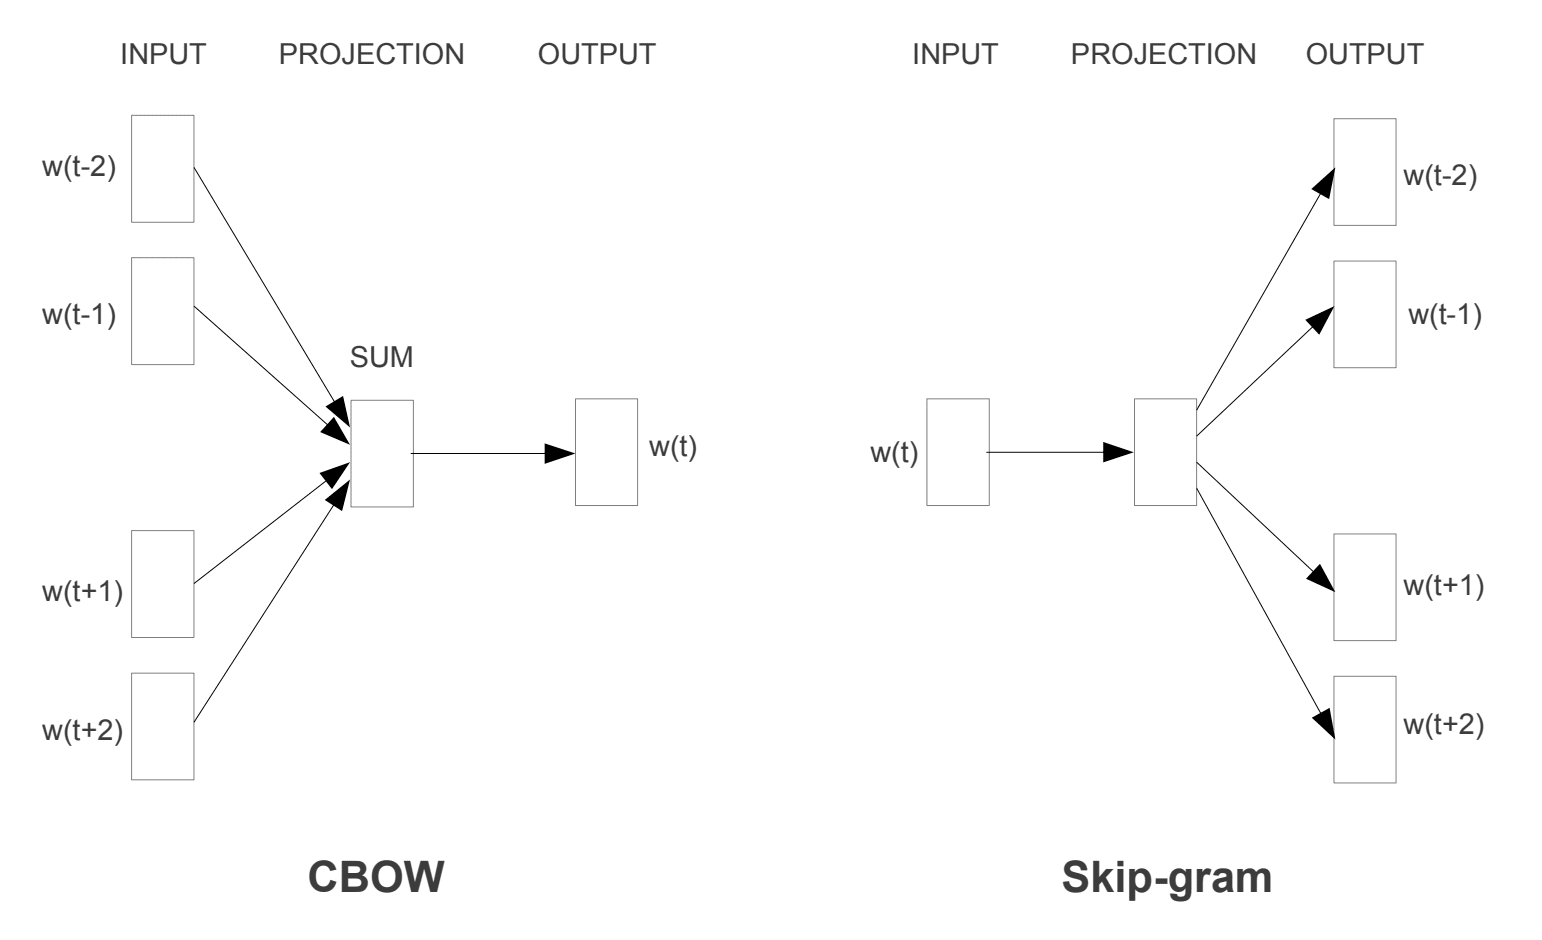
\includegraphics[width=\textwidth]{figures/word2vec-training-models.png}
  \caption[TODO]{TODO: desc}
  \label{fig:word2vec-learning-models}
\end{figure}

The key benefit of the approach is that high-quality word embeddings
can be learned efficiently (low space and time complexity), allowing
larger embeddings to be learned (more dimensions) from much larger
corpora of text (billions of words). Also, Word2Vec perform
significantly better than LSA for preserving linear regularities among
words and LDA moreover becomes computationally very expensive on
large data sets.

\subsection{GloVe}

GloVe is an extension to the Word2Vec method for efficiently learning
word vectors, developed by Pennington \etal{} in \todo{CITE: glove},
that wants to to marry both the global statistics of matrix
factorization techniques like LSA with the local context-based
learning in Word2Vec. Rather than using a window to define local
context, GloVe constructs an explicit word-context or word
co-occurrence matrix using statistics across the whole text corpus.
The result is a learning model that may result in generally better
word embeddings.

\subsection{Other methods}

\newthought{BERT} -- Bidirectional Encoder Representations from Transformers is a relatively recent language representation model, introduced by J. Devlin \etal{} in \todo{CITE: BERT: Pre-training of Deep Bidirectional Transformers for Language Understanding},  designed to pretrain deep bidirectional representations from
unlabeled text by jointly conditioning on both left and right context in all layer. BERT’s key technical innovation is applying the bidirectional training of Transformer, a popular attention model, to language modelling. This is in contrast to previous efforts which looked at a text sequence either from left to right or combined left-to-right and right-to-left training.

\todo{ADD OR REMOVE: Both families suffer significant drawbacks. While methods like LSA efficiently leverage statistical information, they do relatively poorly on the word analogy task, indicating a sub-optimal vector space structure. Methods like skip-gram may do better on the analogy task, but they poorly utilize the statistics of the corpus since they train on separate local context windows instead of on global co-occurrence counts.}

\section{Intersection over Union (IoU)}

Given a pair of bounding box coordinates (b i , b j ), the
Intersection over Union (IoU), also known as Jaccard index, is an evaluation metric used mainly in object detection
tasks, which aims to evaluate how much the two bounding
box refer to the same content in the image. Specifically, it
is defined as:
\[
  \iou(\bbox_i, \bbox_i) = \frac{| \bbox_i \inters \bbox_j |}{| \bbox_i \union \bbox_j |}
\]
where $| \bbox_i \inters \bbox_j |$ is the area of the box obtained by
the intersection of boxes $\bbox_i$ and $\bbox_j$ , while $| \bbox_i
\union \bbox_j |$ is the area of the box obtained by the union of
boxes $\bbox_i$ and $\bbox_j$. It is invariant to the bounding boxes
sizes, and it returns values that are strictly contained in the
interval $[0, 1] \in \Rset$, where $1$ means that the two bounding
boxes refer to the same image area, while a score of $0$ means that
the two bounding boxes do not overlap at all. The fact that two
bounding boxes that do not overlap have IoU score equal to $0$, is the
major issue of this metric: the zero value does not represent how much
the two bounding boxes are far from each other. For this reason, in
its standard definition, the intersection over union is mainly used as
an evaluation metric rather than as a component of a loss function for
learning.
